% Options for packages loaded elsewhere
\PassOptionsToPackage{unicode}{hyperref}
\PassOptionsToPackage{hyphens}{url}
%
\documentclass[
]{article}
\usepackage{amsmath,amssymb}
\usepackage{lmodern}
\usepackage{iftex}
\ifPDFTeX
  \usepackage[T1]{fontenc}
  \usepackage[utf8]{inputenc}
  \usepackage{textcomp} % provide euro and other symbols
\else % if luatex or xetex
  \usepackage{unicode-math}
  \defaultfontfeatures{Scale=MatchLowercase}
  \defaultfontfeatures[\rmfamily]{Ligatures=TeX,Scale=1}
\fi
% Use upquote if available, for straight quotes in verbatim environments
\IfFileExists{upquote.sty}{\usepackage{upquote}}{}
\IfFileExists{microtype.sty}{% use microtype if available
  \usepackage[]{microtype}
  \UseMicrotypeSet[protrusion]{basicmath} % disable protrusion for tt fonts
}{}
\makeatletter
\@ifundefined{KOMAClassName}{% if non-KOMA class
  \IfFileExists{parskip.sty}{%
    \usepackage{parskip}
  }{% else
    \setlength{\parindent}{0pt}
    \setlength{\parskip}{6pt plus 2pt minus 1pt}}
}{% if KOMA class
  \KOMAoptions{parskip=half}}
\makeatother
\usepackage{xcolor}
\usepackage[margin=1in]{geometry}
\usepackage{graphicx}
\makeatletter
\def\maxwidth{\ifdim\Gin@nat@width>\linewidth\linewidth\else\Gin@nat@width\fi}
\def\maxheight{\ifdim\Gin@nat@height>\textheight\textheight\else\Gin@nat@height\fi}
\makeatother
% Scale images if necessary, so that they will not overflow the page
% margins by default, and it is still possible to overwrite the defaults
% using explicit options in \includegraphics[width, height, ...]{}
\setkeys{Gin}{width=\maxwidth,height=\maxheight,keepaspectratio}
% Set default figure placement to htbp
\makeatletter
\def\fps@figure{htbp}
\makeatother
\setlength{\emergencystretch}{3em} % prevent overfull lines
\providecommand{\tightlist}{%
  \setlength{\itemsep}{0pt}\setlength{\parskip}{0pt}}
\setcounter{secnumdepth}{-\maxdimen} % remove section numbering
\usepackage{cancel}
\ifLuaTeX
  \usepackage{selnolig}  % disable illegal ligatures
\fi
\IfFileExists{bookmark.sty}{\usepackage{bookmark}}{\usepackage{hyperref}}
\IfFileExists{xurl.sty}{\usepackage{xurl}}{} % add URL line breaks if available
\urlstyle{same} % disable monospaced font for URLs
\hypersetup{
  pdftitle={Caso Gamma revisto²},
  pdfauthor={Silvaneo Viera dos Santos Junior},
  hidelinks,
  pdfcreator={LaTeX via pandoc}}

\title{Caso Gamma revisto²}
\usepackage{etoolbox}
\makeatletter
\providecommand{\subtitle}[1]{% add subtitle to \maketitle
  \apptocmd{\@title}{\par {\large #1 \par}}{}{}
}
\makeatother
\subtitle{Relatório}
\author{Silvaneo Viera dos Santos Junior}
\date{2022-11-23}

\begin{document}
\maketitle

\hypertarget{priori-alternativa-para-o-modelo-gamma}{%
\subsection{Priori alternativa para o modelo
Gamma}\label{priori-alternativa-para-o-modelo-gamma}}

Neste relatório apresentaremos um \emph{follow-up} das análises feitas
sobre o GDLM k-paramétrico para o caso Gamma com parâmetro de forma e
média desconhecidos. Neste relatório apresento as contas para o ajuste
feito com a parametrização do Bernardo.

Modelo observacional: \[
 X|\phi,\mu \sim \mathcal{G}\left(\phi,\frac{\phi}{\mu}\right)
 \]

Priori:

\[
\begin{aligned}
\pi(\phi,\mu) &\propto \exp\left\{n_0\left(\phi \ln\left(\frac{\phi}{\mu}\right)-\ln(\Gamma(\phi)\right)+\theta_0\phi-\tau_0\frac{\phi}{\mu}\right\}\\
&=\exp\left\{-n_0\left(\phi \ln(\mu)-\ln(\phi)+\ln(\Gamma(\phi)\right)+\theta_0\phi-\tau_0\frac{\phi}{\mu}\right\},
\end{aligned}
\]

Nesta priori, temos que o vetor de estatística suficientes associado é
\(H_{p}=\left(\phi,\frac{\phi}{\mu},\phi\ln(\mu)-\phi\ln(\phi)+\ln(\Gamma(\phi))\right)'\).

Se \(X,Y\) tem densidade \(\pi\), então diremos que
\(X,Y \sim \Pi(n_0,\tau_0,\theta_0)\). Se
\(\phi, \mu \sim \Pi\left(n_0,\theta_0,\tau_0\right)\), então:

\[
\begin{aligned}
f(\mu|\phi)&\propto \pi(\phi,\mu) \propto \exp\left\{-(n_0\phi \ln(\mu)-\phi\ln(\phi)+\ln(\Gamma(\phi))+\theta_0\phi-\tau_0\frac{\phi}{\mu}\right\}\\
& \propto \exp\left\{-n_0\phi \ln(\mu)-\tau_0\frac{\phi}{\mu}\right\}\\
&=\mu^{-n_0\phi}e^{-\tau_0\frac{\phi}{\mu}},
\end{aligned}
\] ou seja \(\mu|\phi \sim \mathcal{IG}(n_0 \phi+1,\phi\tau_0)\), onde
\(\mathcal{IG}\) representa a distribuição Inversa Gamma.

Usando a distribuição condicional de \(\mu\) podemos reescrever
\(\mathbb{E}_{p}[H_{p}]=\mathbb{E}_{p}[\mathbb{E}_{p}[H_{p}|\phi]]\), de
onde obtemos:

\[
\begin{aligned}
\mathbb{E}_{p}\left[\frac{\phi}{\mu}\right]&=\mathbb{E}_{p}[\phi\mathbb{E}_{p}\left[\frac{1}{\mu}|\phi\right]]=\mathbb{E}_{p}\left[\phi\frac{n_0\phi+1}{\phi \tau_0}\right]=\frac{n_0\mathbb{E}_{p}\left[\phi\right]+1}{ \tau_0}\\
\mathbb{E}_{p}[\phi\ln(\mu)]&=\mathbb{E}_{p}[\phi\mathbb{E}_{p}[\ln(\mu)|\phi]]=\mathbb{E}_{p}\left[\phi(-\psi(n_0 \phi +1 )+\ln(\phi\tau_0))\right].
 \end{aligned}
\]

Usando que
\(\mathbb{E}_{p}\left[\phi\right]=\mathbb{E}_q\left[\phi\right]\)
(\(\mathbb{E}_q\left[H_p\right]\) é suposto conhecido), temos que:

\[
\tau_0=\frac{n_0\mathbb{E}_{q}\left[\phi\right]+1}{\mathbb{E}_{q}\left[\frac{\phi}{\mu}\right]}
\]

Ademais:

\[
\begin{aligned}
\mathbb{E}_{p}[\phi\ln(\mu)-\phi\ln(\phi)+\ln(\Gamma(\phi))]&=\mathbb{E}_{p}[\phi\ln(\mu)]+\mathbb{E}[-\phi\ln(\phi)+\ln(\Gamma(\phi))]\\
&=\mathbb{E}_{p}\left[\phi(-\psi(n_0 \phi +1 )+\ln(\phi\tau_0))\right]+\mathbb{E}[-\phi\ln(\phi)+\ln(\Gamma(\phi))]\\
&=\mathbb{E}_{p}\left[-\phi\psi(n_0 \phi +1 )+\phi\ln(\tau_0)+\cancel{\phi\ln(\phi)}-\cancel{\phi\ln(\phi)}+\ln(\Gamma(\phi))\right]\\
&=\mathbb{E}_{p}\left[\ln(\Gamma(\phi))-\phi\psi(n_0 \phi +1 )\right]+\mathbb{E}_q\left[\phi\right]\ln(\tau_0)
 \end{aligned}
\]

Com as equações acimas, conseguimos escrever \(\mathbb{E}_{p}[H_{p}]\)
como valores esperados que dependem apenas da distribuição marginal de
\(\phi\), sendo que a distribuição marginal de \(\phi\) é tal que:

\[
\begin{aligned}
f(\phi)&\propto \int_0^{+\infty}\pi(\phi,\mu) d\mu\\
&\propto \int_0^{+\infty}\exp\left\{-(n_0\phi \ln(\mu)-\phi\ln(\phi)+\ln(\Gamma(\phi))+\theta_0\phi-\tau_0\frac{\phi}{\mu}\right\}d\mu\\
&= \exp\{n_0(\phi\ln(\phi)-\ln(\Gamma(\phi))+\theta_0\phi\}\int_0^{+\infty}\exp\left\{-n_0\phi \ln(\mu)-\tau_0\frac{\phi}{\mu}\right\}d\mu\\
&= \exp\{n_0(\phi\ln(\phi)-\ln(\Gamma(\phi))+\theta_0\phi\}\frac{\Gamma(n_0\phi+1)}{\phi^{n_0\phi+1}\tau_0^{n_0\phi+1}}\\
&\propto \frac{\phi^{n_0\phi}}{\Gamma(\phi)^{n_0}}\frac{\Gamma(n_0\phi+1)}{\phi^{n_0\phi+1}\tau_0^{n_0\phi+1}}\exp\{\theta_0\phi\}\\
&= \frac{\phi^{n_0\phi}}{\phi^{-n_0}\Gamma(\phi+1)^{n_0}}\frac{\Gamma(n_0\phi+1)}{\phi^{n_0\phi+1}\tau_0^{n_0\phi+1}}\exp\{\theta_0\phi\}.
 \end{aligned}
\]

Novamente, a fórmula de Stirling nos diz que:

\[
\Gamma(x+1) \approx \sqrt{2\pi x}\left(\frac{x}{e}\right)^x.
\]

Usando essa aproximação na densidade de \(\phi\) obtemos que:

\[
\begin{aligned}
f(\alpha)&\propto \frac{\phi^{n_0\phi}}{\phi^{-n_0}\Gamma(\phi+1)^{n_0}}\frac{\Gamma(n_0\phi+1)}{\phi^{n_0\phi+1}\tau_0^{n_0\phi+1}}\exp\{\theta_0\phi\}\\
&\approx \frac{\phi^{n_0\phi}}{\phi^{-n_0}(\sqrt{2\pi\phi}(\frac{\phi}{e})^{\phi})^{n_0}}\frac{\sqrt{2\pi n_0\phi}(\frac{n_0\phi}{e})^{n_0\phi}}{\phi^{n_0\phi+1}\tau_0^{n_0\phi+1}}\exp\{\theta_0\phi\}\\
&\propto \frac{\cancel{\phi^{n_0\phi}}}{\phi^{-n_0}\phi^{\frac{n_0}{2}}\cancel{\phi^{n_0\phi}}e^{-n_0\phi}}\frac{n_0^{n_0\phi}\phi^{\frac{1}{2}}\cancel{\phi^{n_0\phi}} e^{-n_0\phi}}{\phi\cancel{\phi^{n_0\phi}}\tau_0^{n_0\phi}}\exp\{\theta_0\phi\}\\
&\propto \phi^{\frac{n_0+1}{2}-1}\exp\{-(n_0\ln\left(\frac{\tau_0}{n_0}\right)-\theta_0)\phi\}.
\end{aligned}
\]

Ou seja, \(\phi\) tem distribuição aproximada
\(\mathcal{G}\left(\frac{n_0+1}{2},n_0\ln\left(\frac{\tau_0}{n_0}\right)-\theta_0\right)\).

A aproximação acima é muito útil para destacar a condição na qual
\(\Pi\) é própria: Para que \(\Pi\), basta que
\(n_0\ln\left(\frac{\tau_0}{n_0}\right)-\theta_0>0\).

Usando a aproximação acima, podemos calcular obter que:

\[
\mathbb{E}_{p}[\phi]=\frac{n_0+1}{2\left(n_0\ln\left(\frac{\tau_0}{n_0}\right)-\theta_0\right)}
\]

Usando que \(\psi(x)\approx \ln(x)-\frac{1}{2x}-\frac{1}{12x^2}\)
(\(\psi\) é a função digamma) e que \(\psi(x+1)=\psi(x)+\frac{1}{x}\),
temos que:

\[
\begin{aligned}
-\phi\psi(n_0\phi+1)&=-\phi\left(\psi(n_0\phi)+\frac{1}{n_0\phi}\right)\\
&\approx-\phi\left(\ln(n_0\phi)-\frac{1}{2n_0\phi}-\frac{1}{12n^{2}_0\phi^2}+\frac{1}{n_0\phi}\right)\\
&\approx-\phi\ln(\phi)-\phi\ln(n_0)+\frac{1}{12n^{2}_0\phi}-\frac{1}{2n_0}.
\end{aligned}
\]

Usando que \(\psi(x)\approx \ln(x)-\frac{1}{2x}-\frac{1}{12x^2}\) junto
ao Teorema Fundamental do Cálculo, obtemos:

\[
\ln(\Gamma(x))= \int^{x}_{1}\psi(t)dt \approx \int^{t}_{1}\ln(t)-\frac{1}{2t}-\frac{1}{12t^2}dt  =\left(t\ln(t)-t-\frac{1}{2}\ln(t)+\frac{1}{12t}\right)^{x}_{1}=x\ln(x)-x-\frac{1}{2}ln(x)+\frac{1}{12x}+\frac{11}{12}
\]

Podemos verificar que a qualidade da aproximação acima no gráfico a
seguir:

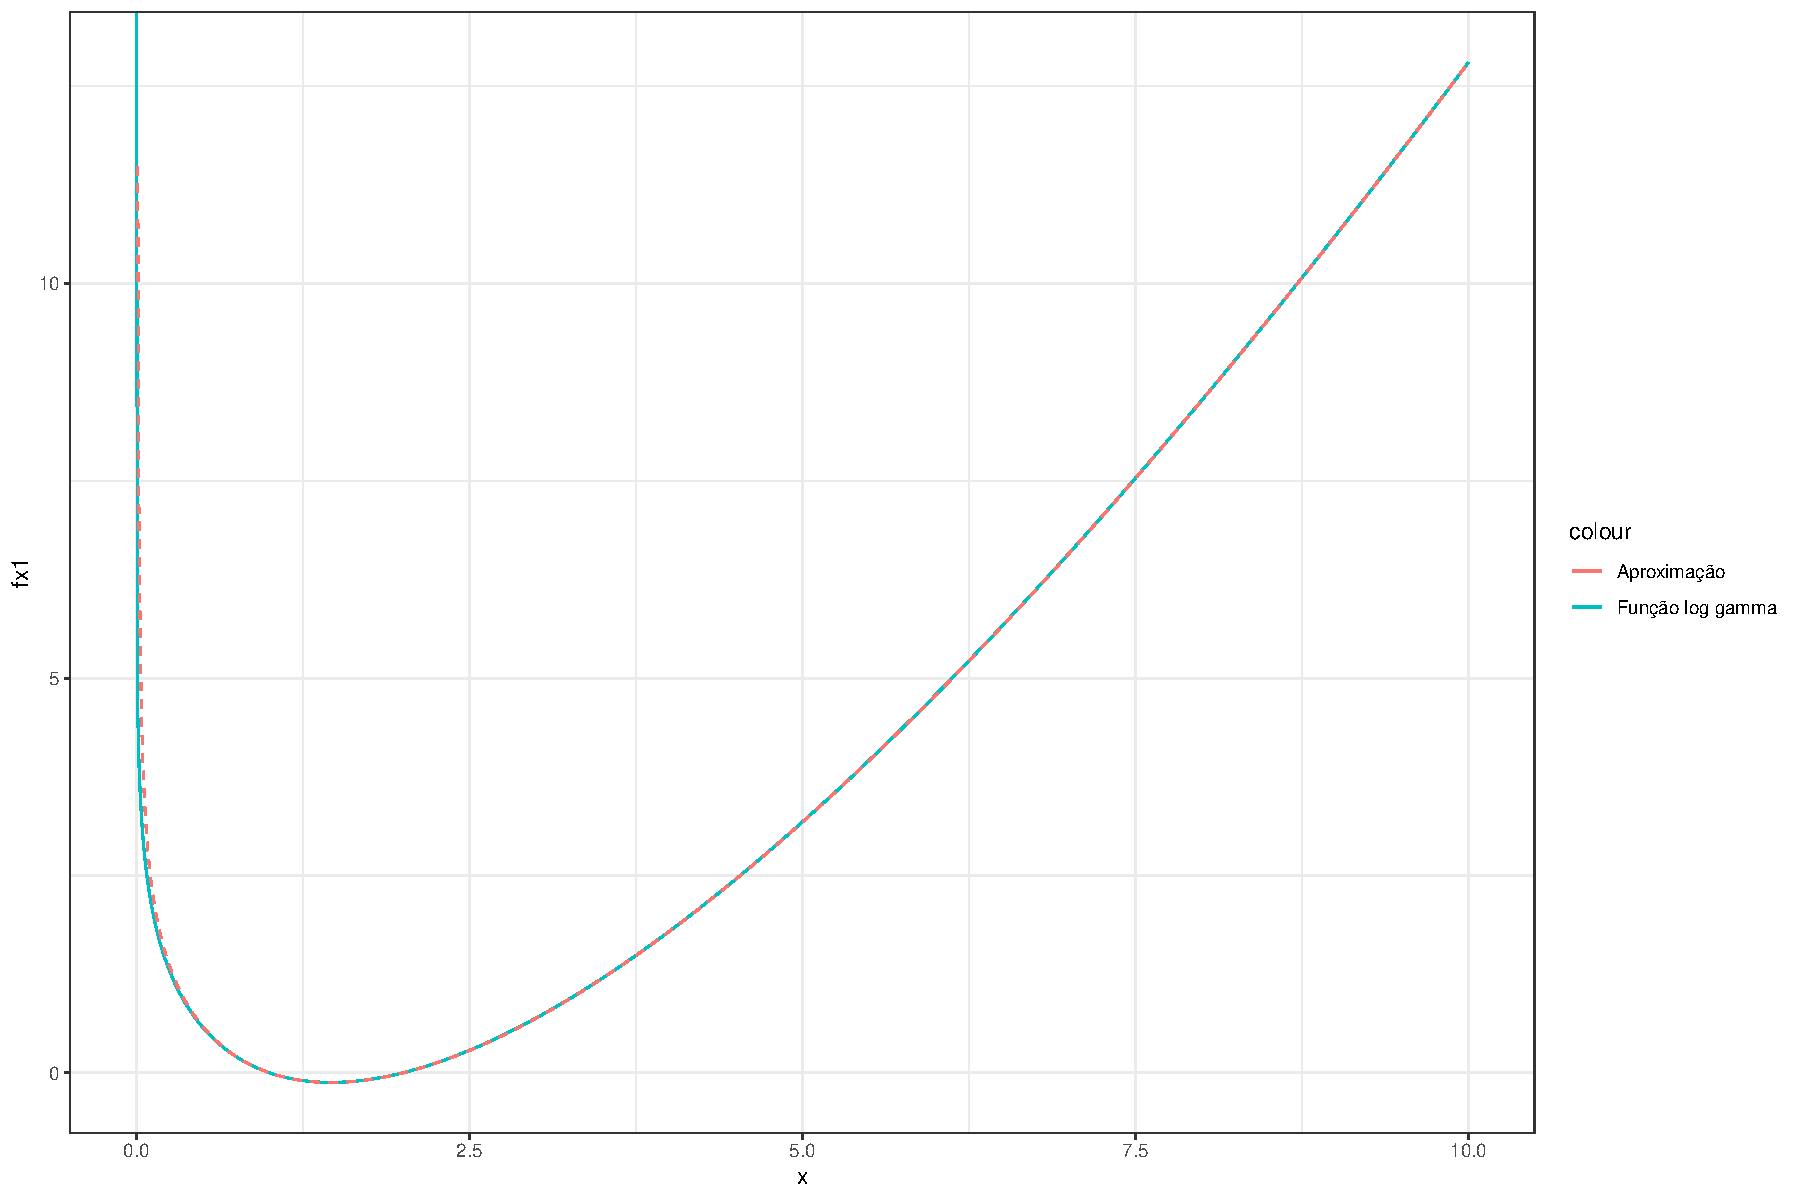
\includegraphics{caso_gamma_revisto_revisto_files/figure-latex/unnamed-chunk-1-1.pdf}

Em geral a aproximação parece boa, porém há certas ressalvas sobre o seu
uso, conforme discutirei mais à frente.

Calculemos então o valor esperado da última estatística suficiente
restante:

\[
\begin{aligned}
\mathbb{E}_{p}[\phi\ln(\mu)-\phi\ln(\phi)+\ln(\Gamma(\phi))]&=\mathbb{E}_{p}\left[\ln(\Gamma(\phi))-\phi\psi(n_0 \phi +1 )\right]+\mathbb{E}_q\left[\phi\right]\ln(\tau_0)\\
&=\mathbb{E}_{p}\left[\cancel{\phi\ln(\phi)}-\phi-\frac{1}{2}ln(\phi)+\frac{1}{12\phi}+\frac{11}{12}-\cancel{\phi\ln(\phi)}-\phi\ln(n_0)+\frac{1}{12n^{2}_0\phi}-\frac{1}{2n_0}\right]\\
&+\mathbb{E}_q\left[\phi\right]\ln(\tau_0)\\
&=-\mathbb{E}_q[\phi](1+\ln(n_0\tau_0))-\frac{1}{2}\psi\left(\frac{n_0+1}{2}\right)\\
&+\frac{1}{2}\ln\left(n_0\ln\left(\frac{\tau_0}{n_0}\right)-\theta_0\right)+\frac{n_0+1}{n_0-1}\frac{\ln\left(\frac{\tau_0}{n_0}\right)-\frac{\theta_0}{n_0}}{6}\\
&+\frac{11}{12}-\frac{1}{2n_0}
\end{aligned}
\] \textbf{A aproximação acima é usada apenas quando \(\frac{n_0+1}{2}\)
é grande (maior que 3 já é o suficiente). Quando \(\frac{n_0+1}{2}\) é
pequeno, esse valor esperado é calculado usando quadratura Gaussiana.}

A expressão aproximada para
\(\mathbb{E}_{p}[\phi\ln(\mu)-\phi\ln(\phi)+\ln(\Gamma(\phi))]\) parece
bastente útil, porém ela tem um defeito muito grave: Ela não são válidas
para \(n_0\le1\). De fato, se \(n_0\le1\), \(\mathbb{E}_{p}[1/\phi]\)
não está definido, o que invalida as equações acima. Vale destacar que
\(\mathbb{E}_{p}[\phi\ln(\mu)-\phi\ln(\phi)+\ln(\Gamma(\phi))]\)
\textbf{existe} e são finitos, porém a aproximação da função \(\psi\) é
ruim para valores baixos de \(n_0\), especificamente, a aproximação de
\(\psi\) é ruim para valores pequenos de \(\phi\) e, quando \(n_0\) é
pequeno, a região onde a aproximação de \(\psi\) é ruim tem bastante
massa de probabilidade, de modo que a aproximação do valor esperado é
ruim.

De todo modo, a observação acima não é necessariamente um empecilho, uma
vez que podemos usar outros métodos para cálcular
\(\mathbb{E}_{p}[\phi\ln(\mu)-\phi\ln(\phi)+\ln(\Gamma(\phi))]\) sem
aproximações.

Usando o novo sistema obtido, tentamos fazer o ajuste do modelo, porém
não conseguimos um ajuste funcional.

\end{document}
